%% ============================================================================
%%
%%  Presentation -- mini-workshop on LaTeX
%%
%%  Author: Jakob Rørsted Mosumgaard
%%
%%  IMPORTANT: Compile with XeLaTeX !
%%
%%  Remarks:
%% - Requires the Fira Sans font family
%% - Needs to be executed with '--shell-escape'
%%
%% ============================================================================

% ~~~~~~~~~~~~~~~~~~~~~~~~~~~~~~~~~~~~~~~~~~~~~~~~~~~~~~~~~~~~~~~~~~~~~~~~~~~~~
% Preamble
% ~~~~~~~~~~~~~~~~~~~~~~~~~~~~~~~~~~~~~~~~~~~~~~~~~~~~~~~~~~~~~~~~~~~~~~~~~~~~~
\documentclass{beamer}

% ~~~~~~~~~~~~~~~~
% Beamer og layout
% ~~~~~~~~~~~~~~~~
 % Use metropolis theme (requires Fira Sans and XeLaTeX / LuaLaTeX)
\usetheme[block=fill]{metropolis}

% Language
\usepackage{polyglossia}
\setdefaultlanguage{danish}

% Typography magic!
\usepackage[final]{microtype}

% Include code with nice and versatile highlighting!
% NOTE: This packages requires the Python-module 'Pygments' to be installes
% NOTE: Fails unless this file is compiled with '--shell-escape' !
\usepackage{minted}
\usemintedstyle{friendly}

% Set beamer font-theme (required for mathspec)
\usefonttheme{professionalfonts}

% Tweak the LaTeX-logo
\usepackage{metalogo}
\setLaTeXa{\scshape a}
\setlogokern{Xe}{-0.061em}
\setlogokern{eL}{-0.057em}
\setlogokern{La}{-0.19em}
\setlogokern{aT}{-0.05em}
\setlogokern{Te}{-0.11em}
\setlogokern{eX}{-0.040em}
\setlogokern{eT}{-0.056em}
\setlogokern{X2}{0.1667em}
\setlogodrop{0.155em}

% Define the alert color from the theme (mLightBrown)
\usepackage{xcolor}
\definecolor{alertcol}{HTML}{EB811B}

% Define background colors for the code highlighting
\definecolor{codebg}{rgb}{0.92,0.92,0.92}
\colorlet{alertbg}{alertcol!30}

% ~~~~~~~~
% Science!
% ~~~~~~~~
% The usual mathematics packages
\usepackage{amsmath}
\usepackage{mathtools}

% Use the theme-font for maths (with weight 'light')
% NOTE: This only works in XeLaTeX (not LuaTeX)!
\usepackage{mathspec}
\setallmainfonts(Digits,Latin){Fira Sans Light}

% Units
\usepackage{siunitx}

% Use correct font for the units as well
% --> Moved to AFTER the document start due to some weird bug...


% ~~~~~~~~~~
% References
% ~~~~~~~~~~
% Quotes
\usepackage{csquotes}

% Webpages
\usepackage{url}

% Smart commands for references
\usepackage{cleveref}

% ~~~~~~
% Macros
% ~~~~~~
% We need this at some point...
\usepackage{xspace}

% Emulate the memoir-command
\newcommand{\plainbreak}[1]{\vspace{#1\baselineskip}}

% Pretty subscript
\newcommand{\var}[2]{\ensuremath{#1_{\textup{#2}}}\xspace}

% Useful repetitions
\newcommand{\mlt}{\ensuremath{\alpha_{\textup{mlt}}}\xspace}
\newcommand{\teff}{\ensuremath{T_{\textup{eff}}}\xspace}
\newcommand{\logg}{\ensuremath{\log g}\xspace}

% Some names
\newcommand{\mystar}{HR~7322\xspace}
\newcommand{\gar}{\textsc{garstec}\xspace}


% ~~~~~~~~~~~~~~~~~~~~~~~~~~~~~~~~~~~~~~~~~~~~~~~~~~~~~~~~~~~~~~~~~~~~~~~~~~~~~
% Document
% ~~~~~~~~~~~~~~~~~~~~~~~~~~~~~~~~~~~~~~~~~~~~~~~~~~~~~~~~~~~~~~~~~~~~~~~~~~~~~
\begin{document}

% This only works after the \begin{document} ???
\sisetup{math-rm=\mathrm}
\sisetup{math-micro=\text{µ},text-micro=µ}


% Now I will start to write in Danish....

% ~~~~~~~~~~~~
% Introduktion
% ~~~~~~~~~~~~

% Definer en titel og indsæt den
\title{Mini-workshop -- \LaTeX{}}
\date{25. september 2017}
\author{Amalie Stokholm \& Jakob Rørsted Mosumgaard}
\institute{STAR -- STuderendes Astronomiske Råd}

% Dette er et titelslide
\maketitle


% Dette er det første slide efter titlen
\begin{frame}
  \frametitle{Om denne mini-workshop}

  \begin{itemize}
  \item Vi antager kendskab til \LaTeX{}
  \item Udvalgte emner
  \item Vores personlige holdninger
  \item Ikke kun \enquote{hård} \LaTeX{}
  \end{itemize}

  \plainbreak1

  \begin{block}{Fokus}
    \begin{itemize}
    \item Interessegruppen i astronomi
    \item Gøre det pænere, men især \alert{nemmere}
    \end{itemize}
  \end{block}
\end{frame}


\begin{frame}
  \frametitle{Oversigt}

  \begin{itemize}
  \item Pakker
  \item Bibliografi
  \item Større projekter
  \item Tips og tricks
  \item Hjælp til selvhjælp
  \end{itemize}

\end{frame}


\begin{frame}
  \frametitle{Løbende workshop}

  Nu: Find jeres seneste \LaTeX-dokument frem og følg med!
\end{frame}


\begin{frame}[standout]
  Brug \  \texttt{memoir} \ som dokumentklasse!
\end{frame}


% ~~~~~~~~~~
% Nyt afsnit
% ~~~~~~~~~~
\section{Pakker}

\begin{frame}[fragile]
  \frametitle{Enheder med \texttt{siunitx}}

  Pakken er klog og \alert{smart}! Den giver konsistente enheder i hele
  dokumentet.

  Man kan eksempelvis skrive:

  {\fontsize{9pt}{11pt}\selectfont
\begin{minted}[bgcolor=codebg]{latex}
a = \SI{1.989e33}{\gram}
b = \SI{9.8}{\meter\per\second\squared}
c = \SI[per-mode=symbol]{9.8}{\meter\per\second\squared}
\end{minted}
    }

    For at få:
  \begin{align*}
    a &= \SI{1.989e33}{\gram} \\
    b &= \SI{9.8}{\meter\per\second\squared} \\
    c &= \SI[per-mode=symbol]{9.8}{\meter\per\second\squared}
  \end{align*}
\end{frame}


\begin{frame}[fragile]
  \frametitle{Enheder med \texttt{siunitx}}

  Den virker også til tal:

  {\fontsize{9pt}{11pt}\selectfont
\begin{minted}[bgcolor=codebg]{latex}
a = \num{1.2e13} \\
b = \num{0.9\pm0.1e-5} \\
c = \num[separate-uncertainty=true]{0.9\pm0.1e-5}
\end{minted}
  }

  Som giver:
  \begin{align*}
    a &= \num{1.2e13} \\
    b &= \num{0.9\pm0.1e-5} \\
    c &= \num[separate-uncertainty=true]{0.9\pm0.1e-5}
  \end{align*}
\end{frame}


\begin{frame}[fragile]
    \frametitle{Enheder med \texttt{siunitx}}

    Eksempel på opsætning i preamble:

    \plainbreak1

\begin{minted}[bgcolor=codebg]{latex}
\usepackage{siunitx}
\sisetup{separate-uncertainty=true}
\DeclareSIUnit\year{yr}
\end{minted}

    \plainbreak1

    Tidligere viste indstillinger kan også sættes \alert{globalt}!

    Og den kan \emph{meget} mere \ldots
\end{frame}


\begin{frame}[fragile]
  \frametitle{Henvisninger med \texttt{cleveref}}

  Her er to henvisninger: figur~\ref{fig:subscript} og \cref{fig:subscript}.

  De er lavet med:

\begin{minted}[bgcolor=codebg]{latex}
figur~\ref{fig:subscript}
og
\cref{fig:subscript}
\end{minted}

  \plainbreak1

  Pakken \alert{finder selv ud af}, hvilken type af objekt der henvises til!

  Og det er nemt at ændre eksempelvis ``figur'' til ``fig.'' eller ``Figur''
  \alert{alle steder} i dokumentet på én gang.
\end{frame}


\begin{frame}[fragile]
    \frametitle{Henvisninger med \texttt{cleveref}}

    Opsætningen er meget nem:

    \plainbreak1

\begin{minted}[bgcolor=codebg]{latex}
\usepackage{cleveref}
\end{minted}

    \plainbreak1

    \alert{Bemærk:} Pakken \texttt{hyperref} kan give problemer! Referencepakker
    skal indlæses \emph{i en bestemt rækkefølge}!
\end{frame}


% ~~~~~~~~~~
% Nyt afsnit
% ~~~~~~~~~~
\section{Bibliografi}

\begin{frame}
  \frametitle{BibLaTeX}

  Vigtigt: Brug \texttt{BibLaTeX} og ikke \texttt{BibTeX}! Pakken er nyere og
  har \emph{mange} indstillingsmuligheder.

  Bemærk dog, at formatet for kilderne er identisk og at de opfører sig ret ens.
  Formatet for kilderne kaldes typisk for \emph{bibtex}.

  \plainbreak1

  Automatisk system til at håndtere kilder, lave \alert{henvisninger} og
  generere en \alert{bibliografi}.

  Det kræver kald af et eksternt program til at oversætte bibliografi-filen til
  noget \LaTeX{} kan læse.

\end{frame}


\begin{frame}[fragile,fragile]
  \frametitle{BibLaTeX}

  Man tilføjer kilder i en såkaldt \texttt{bib}-fil og henviser til dem i
  teksten med:
\begin{minted}[bgcolor=codebg]{latex}
\cite{...}
\textcite{...}
\Textcite{...}
\parencite{...}
\end{minted}

  Når man har henvist til en ny kilde, skal bibliografiprogrammet køres igen.
\end{frame}


\begin{frame}[fragile,fragile]
  \frametitle{Indlæsning af \texttt{biblatex}}

  Simpelt:
\begin{minted}[bgcolor=codebg]{latex}
\usepackage[backend=biber]{biblatex}
\addbibresource{bibliography.bib}
\end{minted}

  Det er \emph{vigtigt} at sætte \alert{backend}!

  Navnet på \texttt{bib}-filen kan selvfølgelig ændres.

  \plainbreak1

  I dokumentet skrives:

\begin{minted}[bgcolor=codebg]{latex}
\raggedyright[4em] \printbibliography
\end{minted}
\end{frame}


\begin{frame}[fragile]
  \frametitle{Indlæsning af \texttt{biblatex} -- flere options}

\begin{minted}[bgcolor=codebg]{latex}
\usepackage[%
backend=biber,
style=authoryear-comp,
sorting=nyt,
sortcites=true,
dashed=false,
maxcitenames=2,
hyperref=true]{biblatex}

\addbibresource{bibliography.bib}

\setlength\bibitemsep{1.5\itemsep}
\DeclareNameAlias{sortname}{last-first}
\end{minted}
\end{frame}


\begin{frame}[fragile]
  \frametitle{Justin?}

  Når pakken indlæses med \texttt{backend=biber}, skal man huske at køre
  \texttt{biber} og \emph{IKKE} \texttt{bibtex} for at generere bibliografien!

  Det kan man sagtens indstille \alert{TeXstudio} til!

  \plainbreak1

  \begin{block}{Typisk workflow når der er en ny kilde}
\begin{minted}{shell}
 pdflatex
 biber
 pdflatex
 pdflatex
\end{minted}
  \end{block}
\end{frame}


\begin{frame}[fragile]
  \frametitle{Selve bib-filen}

  Kilderne organiseres i filen med et bestemt format.

  \plainbreak1

  \begin{exampleblock}{Eksempel på en artikel}
    \fontsize{8pt}{10pt}\selectfont
\begin{minted}{bibtex}
 @ARTICLE{weiss2008,
   author = {{Weiss}, A. and {Schlattl}, H.},
   title = "{GARSTEC -- the Garching Stellar Evolution Code}",
   journal = {Astrophysics and Space Science},
   year = 2008,
   month = aug,
   volume = 316,
   pages = {99-106},
 }
\end{minted}
  \end{exampleblock}
\end{frame}


\begin{frame}[fragile]
  \frametitle{Selve bib-filen}

  \begin{exampleblock}{Eksempel på en bog}
    \fontsize{8pt}{10pt}\selectfont
\begin{minted}{bibtex}
 @BOOK{asteroseismology,
   author = {{Aerts}, C. and {Christensen-Dalsgaard}, J. and
            {Kurtz}, D.~W.},
   title = "{Asteroseismology}",
   series = "Astronomy and Astrophysics Library",
   publisher = "Springer Science+Business Media",
   year = 2010,
 }
\end{minted}
  \end{exampleblock}
\end{frame}


\begin{frame}[fragile]
  \frametitle{Selve bib-filen}

  \begin{exampleblock}{Eksempel på en onlinekilde}
    \fontsize{8pt}{10pt}\selectfont
\begin{minted}{bibtex}
 @ONLINE{kepler,
    author = {{NASA}},
    title = "{Kepler: A Search for Habitable Planets}",
    url = {http://kepler.nasa.gov},
    year = 2014,
    urldate = {2014-06-29},
 }
\end{minted}
  \end{exampleblock}
\end{frame}


\begin{frame}
  \frametitle{Selve bib-filen}

  Indgange kan eksporteres fra et program (eksempelvis Mendeley) eller hentes
  fra nettet.

  Filen må \emph{ikke} indeholde \alert{specialtegn}!

\end{frame}


\begin{frame}
  \frametitle{Find referencer -- ADS}

  \bigskip

  \begin{exampleblock}{StedET at finde astronomiartikler}
    ADS: \url{ui.adsabs.harvard.edu}
  \end{exampleblock}

  \begin{figure}[!h]
    \centering
    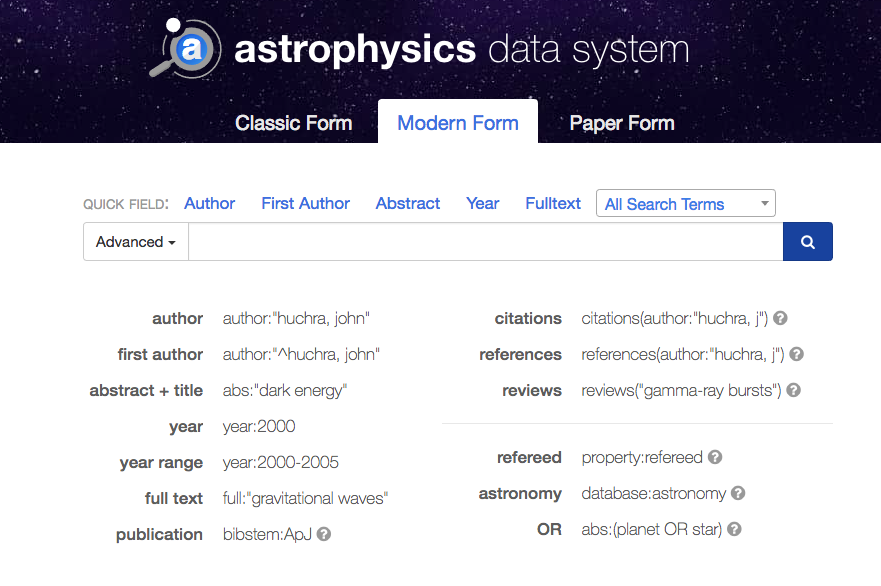
\includegraphics[width=0.85\textwidth]{figures/ads}
  \end{figure}
\end{frame}


\begin{frame}
  \frametitle{Find referencer -- ADS}

  ADS kan mange smarte ting:

  \begin{figure}[!h]
    \centering
    \begin{minipage}{.5\textwidth}
      \centering
      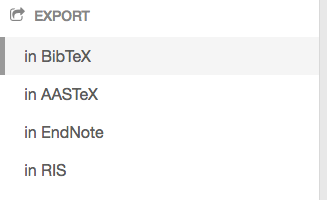
\includegraphics[width=.9\linewidth]{figures/ads_eksport}
    \end{minipage}%
    \begin{minipage}{.5\textwidth}
      \centering
      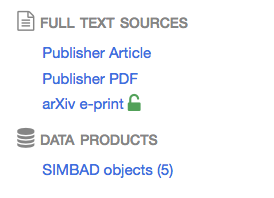
\includegraphics[width=.9\linewidth]{figures/ads_format}
    \end{minipage}
\end{figure}

\end{frame}


\begin{frame}
  \frametitle{Find referencer -- Google Scholar}

  Interaktiv tutorial!

\end{frame}


% ~~~~~~~~~~
% Nyt afsnit
% ~~~~~~~~~~
\section{Større projekter}

\begin{frame}[fragile]
  \frametitle{Opbygning af projekt i flere filer}

  \LaTeX{} kan sagtens arbejde med et projekt i flere filer!

  Man peger compileren på \'{e}n fil, som inkluderer de andre. Denne fil kaldes
  \alert{master-filen}. I TeXstudio kaldes det for \emph{root-document}.

  Eksempelvis kan man have sin preamble i en fil for sig og ellers hvert kapitel
  i sin egen fil.
\end{frame}


\begin{frame}[fragile]
  \frametitle{Opbygning af projekt i flere filer}

    Man kan indsætte sin preamble med

\begin{minted}[bgcolor=codebg]{latex}
\input{preamble}
\end{minted}

  men ellers skal man bruge

\begin{minted}[bgcolor=codebg]{latex}
\include{...}
\end{minted}

  Når man bruger \texttt{include} kommer det på en ny begyndelsesside.
\end{frame}


\begin{frame}[fragile]
  \frametitle{Opbygning af projekt i flere filer}

  Ydermere er \texttt{include} smart, da man så kan nøjes med at compile det
  kapitel man arbejder i:

  \begin{exampleblock}{Fra \texttt{master}-dokumentet}
\begin{minted}{latex}
 % Which files to compile
 \includeonly{%
 %  front/frontpage,
 % chap1/chap1,
   chap2/chap2
 }
\end{minted}
  \end{exampleblock}

    \begin{exampleblock}{Et hack til at inkludere det hele}
\begin{minted}{latex}
 \renewcommand\includeonly[1]{}
\end{minted}
  \end{exampleblock}
\end{frame}


\begin{frame}[fragile,fragile]
  \frametitle{Simpelt eksempel på en master}

  \fontsize{8pt}{10pt}\selectfont

\begin{minted}[bgcolor=codebg]{latex}
\documentclass[11pt, a4paper]{memoir}

\input{preamble}

% Uncomment to include all  -->  Ugly hack, I know !
\renewcommand\includeonly[1]{}

% Which files to compile
\includeonly{%
%  front/frontpage,
%  chap1/chap1,
  chap2/chap2
}

\begin{document}
\include{front/frontpage}
\include{chap1/chap1}
\include{chap2/chap2}
\end{document}
\end{minted}
\end{frame}


\begin{frame}[standout]
  \frametitle{Godt begyndt er halvt fuldendt}

  Find en god preamble!
\end{frame}


\begin{frame}
  \frametitle{Godt begyndt er halvt fuldendt}

  \begin{exampleblock}{Jakobs preamble på GitHub}
    Lavet til et speciale:

    \url{https://github.com/jakobmoss/templates/tree/master/thesis}
  \end{exampleblock}

\end{frame}


% ~~~~~~~~~~
% Nyt afsnit
% ~~~~~~~~~~
\section{Tips og tricks}

% Funktioner
\begin{frame}
  \frametitle{Pæn matematik}
  Hvordan skriver man \alert{korrekt} matematiske funktioner i \emph{math}-mode?

  \begin{align*}
    &\, cos x   &&\, sin x   &&\, exp x   &&\, log x   &&\, ln x
  \end{align*}
  %
  eller
  %
  \alert<2>{
    \begin{align*}
      &\cos x   &&\sin x   &&\exp x   &&\log x   &&\ln x
    \end{align*}
  }
\end{frame}


\begin{frame}[fragile]
  \frametitle{Pæn matematik}
  Hvordan skriver man \alert{korrekt} matematiske funktioner i \emph{math}-mode?

\begin{minted}[bgcolor=codebg]{latex}
\begin{align*}
cos x   sin x   exp x   log x   ln x
\end{align*}
\end{minted}

  eller

\begin{minted}[bgcolor=alertbg]{latex}
\begin{align*}
\cos x   \sin x   \exp x   \log x   \ln x
\end{align*}
\end{minted}
\end{frame}


\begin{frame}
  \frametitle{Pænt subscript}

  Hvordan skriver man tekst i subscript \alert{på en pæn måde}?

    \begin{align*}
      T_{eff}&= \SI{5777}{\kelvin}  && R_{Earth} \simeq \SI{6000}{\kilo\meter}
    \end{align*}
    %
    eller
    %
    \alert<2>{%
      \begin{align*}
        T_{\textup{eff}} &= \SI{5777}{\kelvin} && R_{\textup{Earth}} \simeq \SI{6000}{\kilo\meter}
      \end{align*}
    }

\end{frame}


\begin{frame}
  \frametitle{Pænt subscript}

  Hvordan skriver man tekst i subscript \alert{på en pæn måde}?

  \plainbreak1

  \ldots\ Måske mere tydelige med den \enquote{almindelige} matematikfont:

  \plainbreak1

  \begin{figure}[!h]
    \centering
    
\includegraphics[width=0.7\textwidth]{figures/subscript_math}
    \caption{Eksempel på pæn subscript.}
    \label{fig:subscript}
  \end{figure}
\end{frame}


\begin{frame}[fragile]
  \frametitle{Pænt subscript}

  Hvordan skriver man tekst i subscript \alert{på en pæn måde}?

\begin{minted}[bgcolor=codebg]{latex}
\begin{align*}
T_{eff} = \SI{5777}{\kelvin}
\end{align*}
\end{minted}

  eller

\begin{minted}[bgcolor=alertbg]{latex}
\begin{align*}
T_{\textup{eff}} = \SI{5777}{\kelvin}
\end{align*}
\end{minted}
\end{frame}


\begin{frame}[fragile]
  \frametitle{Pænt subscript}

  Man kan også nemt definere en meget brugbar makro til det:

\begin{minted}[bgcolor=codebg]{latex}
\newcommand{\var}[2]{#1_{\textup{#2}}}
\end{minted}

  \pause

  eller endnu bedre:

  {\fontsize{8pt}{10pt}\selectfont
\begin{minted}[bgcolor=alertbg]{latex}
\newcommand{\var}[2]{\ensuremath{#1_{\textup{#2}}}\xspace}
\end{minted}
  }

  Bemærk pakken \texttt{xspace} som automatisk regner ud, om der skal være et
  mellemrum eller ej!
\end{frame}


\begin{frame}[fragile]
  \frametitle{Makroer}

  Ting man skriver ofte -- eksempelvis \teff, \logg og \mlt -- kan med fordel
  defineres som makroer.

  \plainbreak1

  {\fontsize{8pt}{10pt}\selectfont
\begin{minted}[bgcolor=codebg]{latex}
\newcommand{\mlt}{\ensuremath{\alpha_{\textup{mlt}}}\xspace}
\newcommand{\teff}{\ensuremath{T_{\textup{eff}}}\xspace}
\newcommand{\logg}{\ensuremath{\log g}\xspace}
\end{minted}
  }
\end{frame}


\begin{frame}[fragile]
  \frametitle{Makroer}

  Det kan også være navne der skal skrives på en bestemt måde, som \mystar eller
  \gar.

  \plainbreak1

  {\fontsize{9pt}{11pt}\selectfont
\begin{minted}[bgcolor=codebg]{latex}
\newcommand{\mystar}{HR~7322\xspace}
\newcommand{\gar}{\textsc{garstec}\xspace}
\end{minted}
  }

  \pause

  \plainbreak1

  \alert{Bonus:} Det er nu meget nemt at lave en ændring af \emph{alle
    forekomster} i dokumentet!
\end{frame}


\begin{frame}
  \frametitle{Pæn tekst i align}

  Her er en align med tekst:
  \begin{align*}
    f(x) &= x^{2} - x + 1
    \intertext{så}
    f(2) - 1 &= 2
  \end{align*}
  %
  Her er en pænere align med tekst:
  \begin{align*}
    f(x) &= x^{2} - x + 1
    \shortintertext{så}
    f(2) - 1 &= 2
  \end{align*}
\end{frame}


\begin{frame}[fragile]
  \frametitle{Pæn tekst i align -- koden}

\begin{minted}[bgcolor=codebg]{latex}
Her er en align med tekst:
\begin{align*}
  f(x) &= x^{2} - x + 1
  \intertext{så}
  f(2) - 1 &= 2
\end{align*}
%
Her er en pænere align med tekst:
\begin{align*}
  f(x) &= x^{2} - x + 1
  \shortintertext{så}
  f(2) - 1 &= 2
\end{align*}
\end{minted}
\end{frame}


\begin{frame}
  \frametitle{Pæn tekst i align -- forklaring}

  Brug en af de to kommandoer til at have pæn alignment omkring tekst!

  Brug \mint{latex}|\shortintertext{...}| hvis teksten er kort og ellers brug
  \mint{latex}|\intertext{...}|
\end{frame}


\begin{frame}
  \frametitle{Pæn fremhævet matematik}

  Som I måske også bemærkede: \alert{Ingen blanke linjer omkring align!} Brug
  kommentartegn, hvis I gerne vil have luft i koden.

  \plainbreak1

  Et sidste råd: Fremhævet matematik indgår i teksten, så husk
  \alert{tegnsætning}!

  \begin{exampleblock}{Tegnsætning i matematik}
    Vi har dermed positionen $y$ givet ved
    %
    \begin{align*}
      y = y_{0} + v_{0} t + \frac{1}{2} a t^{2} \; ,
    \end{align*}
    %
    hvor $y_0$ er begyndelsespositionen, $t$ er tiden og \ldots
  \end{exampleblock}
\end{frame}


\begin{frame}[fragile]
  \frametitle{Pæn fremhævet matematik}

  \bigskip

  \begin{exampleblock}{Tegnsætning i matematik}
    Vi har dermed positionen $y$ givet ved
    %
    \begin{align*}
      y = y_{0} + v_{0} t + \frac{1}{2} a t^{2} \; ,
    \end{align*}
    %
    hvor $y_0$ er begyndelsespositionen, $t$ er tiden og \ldots
  \end{exampleblock}

  \begin{exampleblock}{Tegnsætning -- kildekoden}
    \fontsize{8pt}{10pt}\selectfont
\begin{minted}{latex}
 Vi har dermed positionen $y$ givet ved
 %
 \begin{align*}
   y = y_{0} + v_{0} t + \frac{1}{2} a t^{2} \; ,
 \end{align*}
 %
 hvor $y_0$ er begyndelsespositionen, $t$ er tiden og \ldots
\end{minted}
  \end{exampleblock}
\end{frame}


% ~~~~~~~~~~
% Nyt afsnit
% ~~~~~~~~~~
\section{Hjælp til selvhjælp}

\begin{frame}
  \frametitle{Der findes en bog}

  \begin{exampleblock}{Bog skrevet af Lars Madsen (a.k.a. \texttt{daleif})}
    Kan findes her: \url{http://math.au.dk/samarbejde/latex/bog/}
  \end{exampleblock}

  \begin{figure}[!h]
    \centering
    
\includegraphics[width=0.95\textwidth]{figures/latex_intro2}
  \end{figure}
\end{frame}


\begin{frame}[fragile]
  \frametitle{RTFM -- indbygget dokumentation}

  Meget nemt at tilgå den \alert{indbyggede dokumentation}. Kør følgende i en
  terminal for den ønskede pakke:
\begin{minted}[bgcolor=codebg]{shell}
texdoc siunitx
\end{minted}

  \begin{exampleblock}{Visse manualer er lange\ldots}
    \begin{description}
    \item[\texttt{siunitx}] 95 sider
    \item[\texttt{beamer}] 249 sider
    \item[\texttt{biblatex}] 259 sider
    \item[\texttt{memoir}] 609 sider
    \item[\texttt{TikZ}] 1161 sider !
    \end{description}
  \end{exampleblock}
\end{frame}


\begin{frame}
  \frametitle{Kloge folk på nettet}

  På \url{tex.stackexchange.com} findes svar på (næsten) alt!

  \begin{figure}[!h]
    \centering
    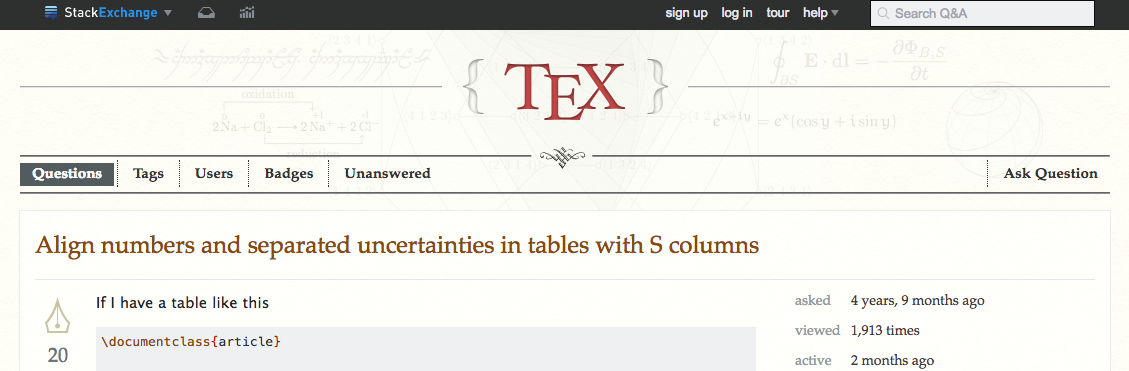
\includegraphics[width=0.95\textwidth]{figures/tex_stack}
  \end{figure}
\end{frame}


\begin{frame}
  \frametitle{Kloge folk på nettet}

  Den nemmeste måde at finde svarene:

    \begin{figure}[!h]
    \centering
    
\includegraphics[width=0.95\textwidth]{figures/tex_google}
  \end{figure}

  Led så efter et passende svar fra \texttt{stackexchange}.
\end{frame}


\begin{frame}
  \frametitle{A final word of caution}

  Pas på hvad du skriver efter \texttt{latex} i et søgefelt!
\end{frame}


% ~~~~~~
% Slut !
% ~~~~~~
\begin{frame}[standout]
  Spørgsmål?
\end{frame}


\begin{frame}[standout]
  \alert{Bonus:} Vi holder en version to af workshoppen når vi kommer nærmere
  bachelorprojekterne!
\end{frame}

\end{document}